\section{Gewonnenen Erkenntnisse}


\subsection{Mathematische Operationen mittels SafeMath}
Arithmetische Operationen in Solidity werden bei einem Überlauf und Unterlauf umgebrochen. Dies kann leicht zu Fehlern führen, da Programmierer normalerweise davon ausgehen, dass ein Überlauf einen Fehler auslöst, was das Standardverhalten in höheren Programmiersprachen ist.

Das folgende Listing \ref{lst:mul} demonstriert das Problem des Überlauf und Unterlauf einer Integer Variable.

\begin{lstlisting}[caption={Beispielhafter Überlauf und Unterlauf},captionpos=b,label=lst:mul]
contract Test {
  function overflow() returns (uint8) {
    uint8 a = 255;
    a = a + 1;  	
    return a; // a = 0
  }
  
  function underflow() returns (uint8) {
    uint8 a = 0;
    a = a - 1;  	
    return a; // a = 255
  }
}
\end{lstlisting}

\subsubsection*{Lösungsansatz}
Durch das explizite prüfen können Überlaufe und Unterläufe erkannt werden und die Transaktion zurückgesetzt werden. Das OpenZeppelin-Framework stellt eine solche Prüfung mittels der SafeMath API zur Verfügung. SafeMath stellt diese Intuition wieder her, indem die Transaktion zurückgesetzt wird, wenn ein Vorgang überläuft. \cite{safemath}

\begin{lstlisting}[caption={Beispielhafte Multiplikation mittels SafeMath zurück},captionpos=b,label=lst:mulsafe]
contract Test {
 using SafeMath for uint8;

 function multiplySafe(uint8 a) returns (uint8) {
   return a.mul(a); // revert() transaction on overflow / underflow
 }
}
\end{lstlisting}


\subsection{Gleitkommaoperationen}
Die Programmiersprache Solidity unterstützt Gleitkommaoperationen nach IEEE 754 nicht. Es gibt jedoch teilunterstützung für Bruchwerte die bestimmten Einschränkungen unterworfen sind.\cite{fixedpointnumbers}

\subsubsection*{Lösungsansätze}

\paragraph*{}
Anstelle von Gleitkommaoperationen, können alternativ entsprechend große Ganzzahlen verwendet werden. Als Beispiel dient z.B. die native Kryptowährung ETH der Ethereum Blockchain. Ein ETH ist eine 19-stellige Ganzzahl. Die kleinste Einheit ist 1 WEI. Ein ETH ist gleich 1.000.000.000.000.000.000 WEI. Durch diese Darstellung können auch Bruchteile eines ETH transferiert werden.

Der Rentenartfaktor (RAF) der Rentenformel ist als Gleitkommazahl definiert und kann Werte von 0 bis 1 annehmen. \cite{raf}

Gleitkommazahlen können auch in diesem Fall durch entsprechend große Ganzzahlen repräsentiert werden, indem im SmartContract immer mit dem Faktor 1000 multipliziert wird. Externe Systeme wie z.B. eine Webanwendung können die Höhe der monatlichen Rente errechnen, indem der Wert entsprechend durch den Devisor 1000 geteilt wird.

\begin{lstlisting}[caption={Verzicht von Gleitkommazahlen durch Multiplikation},captionpos=b,label=lst:simfloat]
contract Rentenformel {
 function rechneBeispiel() returns (uint256) {
   uint256 ep = 40;
   uint256 zf = 1;
   uint256 raf = 250; // kleine Witwenrente = 0.25 * 1000
   uint256 arw = 30;
   
   uint256 mtlRente = ep * zf * raf * arw; // mtlRente = 300000;
   
   return mtlRente; 
   // Extern z.B. in Webanwendung: mtlRente / 1000 = 300
 }
}
\end{lstlisting}

\paragraph*{}
Alternativ kann auf Bibliotheken wie z.B. DS-Math \footnote{\url{https://github.com/dapphub/ds-math}} zurückgegriffen werden, welche entsprechende Funktionalitäten bieten


\subsection{Zeitkomplexität von Smart Contract Methoden}

Jede Ethereum-Transaktion (somit auch jede Ausführung einer Smart Contract Methode) verbraucht "Gas". Pro Transaktion steht nur eine bestimmte Menge an Gas zur Verfügung. Somit sind die Ausführungszeiten und die Aufgaben, welche inerhalb einer Smart Contract Methode ausgeführt werden können, ebenfalls begrenzt. 
Verbraucht eine Ethereum-Transaktion zu viel Gas, wird die Transaktion abgewiesen und nicht in die Blockchain mit aufgenommen.

\subsubsection*{Lösungsansatz}
Die Zeitkomplexität\footnote{\url{http://www.inf.fu-berlin.de/lehre/SS12/ALP2/slides/V6_Rekursion_vs_Iteration_ALP2.pdf}} von SmartContract Methoden sollte immer konstant sein (O(1)). Zeitkomplexität kann reduziert werden, in dem Daten vorberechnet und aggregiert werden.

\paragraph*{} 
Statt wie in Listing \ref{lst:complexitybad} über eine Liste aller Beitragszahlungen zu iterieren, kann die Gesamtsumme aller Beitragszahlungen schon in zahleBeitrag aggregiert werden, sodass die Zeitkomplexität immer O(1) ist.

\begin{lstlisting}[caption={Schlecht - Zeitkomplexität von summeBeitragszahlungen() ist O(n)},captionpos=b,label=lst:complexitybad]
contract Rente {
 uint256[] beitragszahlungen;

 function zahleBeitrag(uint256 beitrag) public {
	beitragszahlungen.push(beitrag);
 }
 
 function summeBeitragszahlungen() public returns (uint256) {
	uint256 summe = 0;
	for (var i = 0; i < beitragszahlungen.length; i++) {
      summe += beitragszahlungen[i];
	}
	return summe;	
 }
}
\end{lstlisting}


\begin{lstlisting}[caption={Gut - Zeitkomplexität von summeBeitragszahlungen() ist O(1)},captionpos=b,label=lst:complexitygood]
contract Rente {
 uint256[] beitragszahlungen;
 uint256 summe;

 function zahleBeitrag(uint256 beitrag) public {
	beitragszahlungen.push(beitrag);
	summe += beitrag;
 }
 
 function summeBeitragszahlungen() public returns (uint256) {
	return summe;	
 }
}
\end{lstlisting}


\subsection{Weitere Beschränkungen bzgl. Smart Contract Programmierung}

\paragraph*{}
Solidity unterstüzt nur statische Zeichenketten. Dynamische Operationen wie das Zusammensetzen von Zeichenketten ist somit ohne weiteres nicht möglich.

\paragraph*{}
Die größe von Smart Contract Quellcode, welche mit einer Transaktion veröffentlicht werden kann, ist beschränkt. Ggf. müssen Zusammenhängende Smart Contract Systeme auf mehrerer Transaktionen aufgeteilt und veröffentlicht werden.

\paragraph*{}
Das Hinterlegen von Smart Contract Quellcode in  Blockchain Explorer (Etherscan.io) ist noch nicht in Truffle integriert und muss händisch durchgeführt werden.


\subsection*{Codeänderungen (Bugfixes und Features)}
Bereitgestellter Smart Contracts Code ist unveränderbar auf der Blockchain gespeichert
Änderungen müssen im Zuge von Fehlerbehebungen und Anforderungsänderungen durchgeführt werden können.

\subsubsection*{Lösungsansatz: Upgradeability Proxy Muster}

\begin{figure}[H]
    \centering
    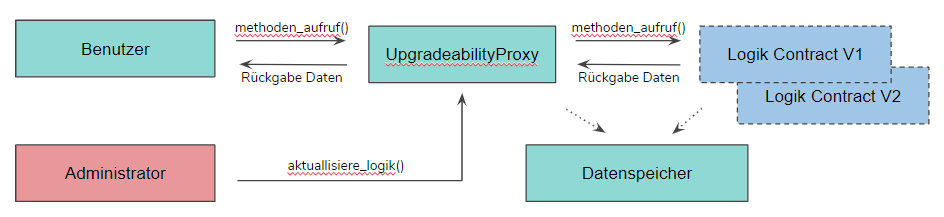
\includegraphics[width=6.0in]{images/pattern-upgrade.png}
    \caption{Smart Contract Upgrade Pattern}
    \label{fig:asure_architecture}
\end{figure}

\subsection*{Abfragen von Blockchain Daten}
Ethereum Smart Contracts bieten nur eine primitive Datenhaltung und rudimentäre Datenabfrage durch Drittanwendungen. 
Benutzer Masken benötigen viele HTTP-Anfragen um die benötigten Daten aus Ethereum in die Anwendung zu laden. 

\paragraph*{}
Eine weitere Herausforderung hinsichtlich der Benutzerführung sind die langen Ausführungszeiten von Transaktionen. Im Durchschnitt wird alle 15 Sekunden ein neuer Ethereum Block in die Blockkette aufgenommen. Dies hat zur Folge, das Transaktionen entsprechend 15 Sekunden oder länger benötigen bis Sie in die Blockchain aufgenommen werden. Ladeanimationen über einen Zeitraum von  mehreren Sekunden sind aus Benutzerperspektive eher suboptimal.

\subsubsection*{Lösungsansatz}
Auf das direkte Abfragen von Blockchain-Daten mittels RPC/HTTP-Schnittstelle verzichten. Stattdessen kann z.B. eine besser geeignete Abfragesprache wie z.B. GraphQL\footnote{\url{https://graphql.org/}} verwendet werden. Die Ethereum Software Geth unterstützt die Abfragesprache GraphQL z.B. seit der Version 1.9.0 nativ \cite{geth}.

Alternativ gibt es spezialisierte Abfrage Proxies z.B. mittels GraphQL wie EthQL\footnote{\url{https://github.com/ConsenSys/ethql}} und TheGraph\footnote{\url{https://thegraph.com/}}.

\paragraph*{}
Durch die Verwendung des Anwendungsmusters Optimistic UI geht die Oberfläche davon aus, dass die entsprechende Schreiboperation erfolgreich war, bevor die Antwort bekannt ist. \cite{optimisticui} Hierdurch entfällt das Anzeigen einer Ladeanimation. Für den Fall, dass die Operation nicht erfolgreich war, muss der Nutzer entsprechend informiert werden.

\paragraph*{}
Eine weitere sinnvolle Lösung kann darin bestehen, Daten niemals direkt von der Blockchain zu lesen, sondern stattdessen eine für Lesezugriffe optimierte Datenbasis aufzubauen. Dieses Vorgehen ist auch als Command-Query-Responsibility-Segregation (CQRS) - Entwurfsmuster bekannt \cite{cqrs}. 


\subsection*{Batch-Job Verarbeitung}
Ethereum bietet keine native Unterstützung für “zeitgesteuerte” Transaktionen.
Ethereum Smart Contracts können nicht direkt auf Smart Contract Ereignisse reagieren.

\subsubsection*{Lösungsansatz}
Externe Systeme können zeitgesteuert und auf Smart Contract Events reagieren - Die Lösung setzt voraus, dass einem externen System “vertraut” wird.


\subsection*{Anbindung externer Datenquellen}
Smart Contracts können nicht direkt auf externe Systeme zugreifen (z.B. mittels HTTP)

\subsubsection*{Lösungsansatz}
Als Lösung bieten sich sogenannte Orakel (Oracles) an. Diese stellen die Daten auf der Blockchain zur Verfügung und stellen auf Anfrage weitere bereit. Es gibt Oracle-Anbieter\footnote{z.B. Chainlink \url{https://chain.link/} und Provable \url{http://provable.xyz/}}, die dies notwendige Infrastruktur bereitstellen und welche als Dienstleistung genutzt werden können. Entwicklung projektbezogener Orakel ist eine weitere Option.

%\subsection*{Wallet Integration}
%Wallet Connect